%   % !TEX root = ../../VIII,3_Rahmen-TeX_9-0.tex
%  
%   Band VIII, 3 N.~?? 	Stoß			(Unter)rubrik			??
%   Signatur/Tex-Datei:	LH_37_05_146-147
%   RK-Nr. 	57273 
%   WZ: 	Bl. X, Nr. 803004
%   edlabels:			21
%   Diagramme: 		1 gültig; 1 gestrichen; 1 mit 1 gestr. + 1 gült. Fassung
%   Dateien (PDF):
%   		LH_37_05_146-147_d1_146r;
%   		LH_37_05_146-147_d2_146r;
%   		LH_37_05_146-147_d3_146r;	eigtl. Fig 3a
%   		LH_37_05_146-147_d4_146r;	eigtl. Fig 3b
%
%   Erstaufnahme:			Krayer 2018
%   Bearbeitung MS ab: 		August 2020
%
%
%
%
\selectlanguage{ngerman}
\frenchspacing
%
\begin{ledgroupsized}[r]{120mm}
\footnotesize
\pstart
\noindent\textbf{Überlieferung:}
\pend
\end{ledgroupsized}
%
\begin{ledgroupsized}[r]{114mm}
\footnotesize
\pstart \parindent -6mm
\makebox[6mm][l]{\textit{L}}%
Konzept:
LH~XXXVII~5~Bl.~146\textendash147. 
Ein Bogen~4\textsuperscript{o};
Wasserzeichen;
Papiererhaltungsmaßnahmen.
Vier Seiten;
Textfolge: 
Bl.~146~r\textsuperscript{o}, Bl.~147~v\textsuperscript{o}, Bl.~147~r\textsuperscript{o}, Bl.~146~v\textsuperscript{o}; im Falzbereich von Bl.~146~v\textsuperscript{o} und Bl.~147~r\textsuperscript{o} mehrere Randanmerkungen.
Der Übergang von Bl.~147~v\textsuperscript{o} zu Bl.~147~r\textsuperscript{o} ist durch den Hinweis \glqq vertatur\grqq\ auf S.~\refpassage{37_05_146-147_18b}{37_05_146-147_18b} gesichert; es folgen auf Bl.~147~r\textsuperscript{o} zwei Anläufe, wovon der zweite durch das Verweiszeichen $\astrosun$ eingeführt wird (S.~\refpassage{37_05_146-147_19}{37_05_146-147_19}).
%
Auf Bl.~147~v\textsuperscript{o} (S.~\refpassage{37_05_146-147_15a}{37_05_146-147_15b}) eigenhändiger Text ohne erkennbaren Bezug zum Stück: \textit{20~D.} \lbrack/\rbrack\ \textit{2.~maß} \lbrack/\rbrack\ \textit{1~lin.}
\pend
\end{ledgroupsized}
%
\begin{ledgroupsized}[r]{114mm}
\footnotesize
\pstart
\parindent -6mm
\makebox[6mm][l]{\textit{E}}%
(tlw.) \cite{01056}\textsc{Fichant} 1994, S.~390f.
\pend%
\end{ledgroupsized}
%
%
\count\Bfootins=1100%
\count\Afootins=1100%
\count\Cfootins=1100
\vspace{5mm}
\begin{ledgroup}
\footnotesize
\pstart
\noindent%
\textbf{Datierungsgründe:}
%%
%
Leibniz führt im vorliegenden Konzept
%
den Begriff des \textit{centrum potentiae} ein,
%
den er für den geraden Stoß zweier gleichförmig bewegter Körper
%
analog zum Schwerpunkt (\textit{centrum gravitatis}) definiert.
%
Das \textit{centrum potentiae} zweier Körper ist demnach
%
der Punkt auf der Stoßlinie, dessen Entfernungen zu den Körpern in umgekehrtem Verhältnis
%
zu den Bewegungsgrößen ($mv$) stehen. 
%
Gleichzeitig mit der Einführung des Begriffs behauptet Leibniz (ohne Beweis),
%
dass die Bewegung des \textit{centrum potentiae} beim Stoß eine  gleichförmige geradlinige ist.
%
Diese These soll wohl eine weitere wichtige Gesetzmäßigkeit von Stoßvorgängen darstellen,
%
über die von \protect\index{Namensregister}{\textso{Huygens} (Hugenius, Ugenius, Hugens, Huguens), Christiaan 1629\textendash1695}Huygens 
%
festgestellte 
%
(\protect\vphantom)\cite{00529}\glqq Regles du mouvement dans la rencontre des corps\grqq, \cite{00157}\textit{JS}, Pariser Ausgabe, 18.~März 1669, hier S.~23f.\protect\vphantom()
%
und von Leibniz selbst übernommene gleichförmige Bewegung des Schwerpunkts hinaus.
%
Die These spielt in den Konzepten N.~\ref{RK57274} 
%
(ebenfalls Mai bis Mitte Juni 1677) 
sowie N.~\ref{RK57277} und N.~\ref{RK57275} (Ende Juni 1677 bis Januar 1678)
eine bedeutende Rolle, wobei sie sich in letzterem Stück schließlich als unhaltbar erweisen wird.
%
%
Daraufhin bestimmt Leibniz, von den Bewegungen der Körper ausgehend,
%
die Lage des \textit{centrum potentiae} vor dem Stoß in drei möglichen Fällen 
%
(siehe bspw.\ S.~\refpassage{37_05_146-147_17a}{37_05_146-147_17b}).
%
Zuletzt widmet er sich einer ausführlichen Berechnung der algebraischen Verhältnisse der Quadrate der Geschwindigkeiten der Körper,
%
wobei er zunächst durch Verwendung der \textit{signa ambigua} alle drei Fälle in einer Gleichung zusammenfasst
%
und sich anschließend (in zwei Anläufen) um eine Vereinfachung der Vorzeichen bemüht.
%
Leibniz gelingt der Nachweis, dass die Gleichung in allen möglichen Fällen dieselben Vorzeichen hat
%
(siehe z.B.\ S.~\refpassage{37_05_146-147_18a}{37_05_146-147_18b}).
%
Die naheliegende physikalische Interpretation dieser allgemeinen Formel,
%
die auch in späteren Konzepten wieder aufgegriffen wird 
%
(siehe N.~\ref{RK60344_2}  und N.~\ref{RK57275}),
%
ist der Erhaltungssatz der kinetischen Energie beim Stoß;
%
diesen wird Leibniz allerdings nach heutigem Kenntnisstand 
%
erst in der \textit{Scheda octava} \textit{De corporum concursu} 
%
(N.~\ref{dcc_08} von Januar 1678, S.~\refpassage{LH_37_05_086r_aequatioinfall-1}{LH_37_05_086r_aequatioinfall-1}),
%
im Rahmen der Einführung des quadratischen Kraftmaßes ($mv^2$), thematisieren.
%
\pend
%
\pstart
Zur Datierung von N.~\ref{RK57273} kann zunächst festgestellt werden, dass
%
die Einführung des \textit{centrum potentiae} am Anfang des Stücks der Struktur
%
von N.~\ref{RK57268} (Mai 1677) nachempfunden ist.
%
Dort ging Leibniz ebenfalls von den zwei Grundregeln der Erhaltung der \glqq directio totalis\grqq\ 
%
und der \glqq potentia totalis\grqq\  beim Stoß aus, wobei in N.~\ref{RK57268} die erste Regel mit 
%
der gleichförmigen Bewegung des Schwerpunkts gleichgesetzt war,
%
hier hingegen die gleichförmige Bewegung des \textit{centrum potentiae} beinhaltet.
%
Möglicherweise stellt N.~\ref{RK57273} den Versuch dar, den
%
(nach Leibnizens Einschätzung sehr erfolgreichen, siehe die Datierungsgründe) Ansatz von  N.~\ref{RK57268}
%
auf den neuen Begriff \textit{centrum potentiae} anzuwenden.
%
Hinzu kommt, dass Leibniz an dieser Stelle einige Ergebnisse von N.~\ref{RK57266-3} (März 1677) und N.~\ref{RK57268} (Mai 1677) rekapituliert, 
%
wie z.B.\ den Lehrsatz \glqq mutationes celeritatum sunt corporibus reciproce proportionales\grqq\ 
%
(siehe S.~\refpassage{37_05_146-147_21a}{37_05_146-147_21b}).
%
Aus diesen Gründen erscheint eine Abfassung von N.~\ref{RK57273} 
%
nach N.~\ref{RK57268}, also ab Mai 1677, sehr wahrscheinlich.
%
\pend
%
\pstart
Von den zwei Konzepten über das \textit{centrum potentiae}, die die Merkmale einer Einführung aufweisen, 
%
ist das vorliegende höchstwahrscheinlich das frühere.
%
Dies geht aus einer Passage des zweiten Stücks (N.~\ref{RK60344_1}) hervor,
%
worin Leibniz sich anschickt, die möglichen Lagen des \textit{centrum potentiae} vor und nach dem Stoß
%
zu bestimmen und dabei auf eine frühere Untersuchung anspielt, 
%
die sich auf seine Lagen vor dem Stoß beschränkt hatte
%
(S.~\refpassage{37_05_152r_7a}{37_05_152r_7b}).
%
Die Beschreibung trifft auf das Konzept N.~\ref{RK57273} zu, welches daher bei der Abfassung von N.~\ref{RK60344_1} vorgelegen haben muss.
%%
\pend
%
\pstart
Zur weiteren Einkreisung der Entstehung von N.~\ref{RK57273} kann das Konzept N.~\ref{RK57274} herangezogen werden.
%
Dieses ist (neben N.~\ref{RK57277} und N.~\ref{RK57275}) eins der Stücke der Jahre 1677\textendash1678, die 
sich auf den Begriff und die Eigenschaften des \textit{centrum potentiae} berufen.
%
Als Terminus ante quem für N.~\ref{RK57274} kann  Mitte Juni 1677 ermittelt werden (siehe die Datierungsgründe). 
%
Unter der Annahme, dass die grundlegenden Ausführungen von N.~\ref{RK57273} 
%
(und N.~\ref{RK60344_1}) der Abfassung von N.~\ref{RK57274} vorausgingen, 
%
kann der genannte Terminus ante quem übernommen werden,
%
woraus sich für N.~\ref{RK57273} die vorgeschlagene Datierungsspanne ergibt.
\pend 
\end{ledgroup}
%%
\selectlanguage{latin}
\frenchspacing
% \newpage%
\vspace{8mm}
\pstart%
\normalsize%
\noindent%
\lbrack146~r\textsuperscript{o}\rbrack\
\pend %Wenn Überschrift/Diagramm
%
%
\vspace{1.0em} %%%%%%%%% Diagramm 1
\centerline{%
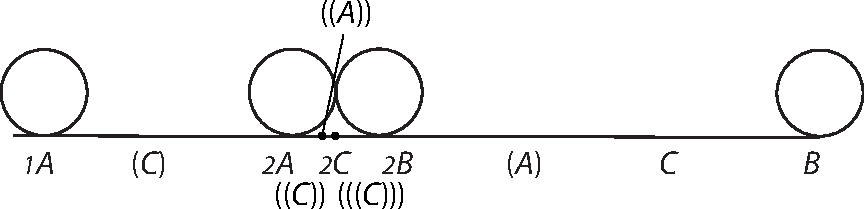
\includegraphics[width=0.78\textwidth]{%
gesamttex/edit_VIII,3/images/LH_37_05_146-147_d1_146r.pdf%
}} 
\vspace{0.5em}
\centerline{%
\lbrack\textit{Fig.~1}\rbrack}
% \newpage%
\vspace{1.5em}
%
\pstart\noindent
%
\edtext{}{% B-Footnote Variante innerhalb Tabelle
{\xxref%
{37_05_146-147_12a}{37_05_146-147_12b}}%
\lemma{\textit{m}}%
\Bfootnote{%
\textit{(1)}~Potentia corporis \textit{a}. %
\textit{(2)}~\dots\ \textit{a}~\textit{L}}}%
%
\par\centering
\begin{edtabularc}%{llllll}
Corporis & \textit{a} & celeritas prior & \textit{e} & posterior & \textit{i} \\
\dots & \textit{b} & celeritas prior & \textit{f} & \dots & \edlabel{37_05_146-147_12a}\textit{m} \\
\dots & \textit{a}\edlabel{37_05_146-147_12b} & potentia \dots & \textit{ae} & \dots & \textit{ai} \\
 & \textit{b} & & \textit{bf} &  & \edlabel{37_05_146-147_1a}\textit{bm}
\end{edtabularc}%
\pend
%
%
\pstart
\edtext{}%
{\xxref{37_05_146-147_1a}{37_05_146-147_1b}%
\lemma{\textit{bm}}%
\Bfootnote{%
\textbar\ 
\textit{(1)}~\textit{{\scriptsize1}B} dexterior quam \textit{{\scriptsize1}C} et \textit{{\scriptsize1}C} dexterior quam \textit{{\scriptsize1}A} 
\textit{(2)}~Si \textit{{\scriptsize1}B} \lbrack...\rbrack\ \textit{{\scriptsize2}B} sequitur 
\textit{(a)}~\textit{{\scriptsize2}B} 
\textit{(b)}~\textit{{\scriptsize2}C}. \textit{erg.}~\textbar\ In \textit{(1)}~con \textit{(2)}~\textbar\ de \textit{streicht Hrsg.}~\textbar\ \textit{(3)}~duorum~\textit{L}}}%
Si
%
\textit{{\scriptsize1}B} dexterior quam \textit{{\scriptsize1}C}, ergo et \textit{{\scriptsize1}B} dexterior quam \textit{{\scriptsize1}A}, et \textit{{\scriptsize2}B} dexterior quam \textit{{\scriptsize2}A}, ergo et \textit{{\scriptsize2}B} dexterior quam \textit{{\scriptsize2}C}, ergo si motus sit a dextro in sinistrum, tunc si \textit{B} sequitur \textit{{\scriptsize1}C}, ergo et \textit{{\scriptsize2}B}
%
sequitur \textit{{\scriptsize2}C}.
%
\pend
\newpage \pstart
%
In duorum\edlabel{37_05_146-147_1b}
%
corporum 
%
\edtext{concursu\protect\index{Sachverzeichnis}{concursus} aio}{\lemma{concursu}\Bfootnote{\textit{(1)}~pono \textit{(2)}~aio~\textit{L}}}
%
servari tum potentiam\protect\index{Sachverzeichnis}{potentia totalis} 
\edtext{\lbrack to\rbrack talem}{\lemma{}\Bfootnote{talem \textit{\ L ändert Hrsg.}}}
tum directionem
% =
totalem.\protect\index{Sachverzeichnis}{directio totalis}%
\pend
%
\pstart
\centering%
\textso{ob Potentiam:}\protect\index{Sachverzeichnis}{potentia}%
%
\pend
%
\pstart
Quia eadem esse debet prior et 
% =
posterior summa potentiarum.\protect\index{Sachverzeichnis}{summa potentiarum}
% = 
Hinc
% = 
\pend
%
\pstart
\centering
$ae + bf \ \displaystyle\overset{(1)}{\sqcap}\ ai + bm$\rule[0cm]{0mm}{12pt}
%
\pend
%
\pstart\noindent
seu
%
$\displaystyle\frac{a}{b}\ \displaystyle\overset{(2)}{\sqcap}\ \displaystyle\frac{m-f}{e-i}$.
%
\edlabel{37_05_146-147_21a}\edtext{Seu mutationes celeritatum\protect\index{Sachverzeichnis}{mutatio celeritatis} sunt corporibus reciproce proportionales.\edlabel{37_05_146-147_21b}
%
$\displaystyle\frac{me-fe}{ef-if}\ \sqcap\ \displaystyle\frac{ae}{bf}$.
Ergo
$\displaystyle\frac{+me\,\protect\ovalbox{$-fe+fe$}-if}{ef-if}\ \sqcap\ \displaystyle\frac{ae+bf}{bf}$
seu
%
$\displaystyle\frac{me-if}{ae+bf\ \sqcap\ ai+bm}\ \sqcap\ \displaystyle\frac{e-i}{b}$.}%
{\lemma{Seu}\Bfootnote{mutationes \lbrack...\rbrack\  $\displaystyle\frac{e-i}{b}$. \textit{erg.}~\textit{L}}} 
% =
\pend
%
\pstart
\noindent 
Unde 
\rule[0cm]{0mm}{12pt}si $e\ \groesser\ i$ erit $f\ \kleiner\ m$
%
\pend
%
\pstart\noindent
seu si prior celeritas major posteriore in uno corpore, erit
minor in altero. Seu si celeritas unius minuitur, celeritas
alterius augetur.
\pend
%
\pstart
\centering\textso{ob Directionem}\protect\index{Sachverzeichnis}{directio}
%
\pend
%
\pstart
Debet centrum potentiae\protect\index{Sachverzeichnis}{centrum potentiae} semper procedere uniformiter.\protect\index{Sachverzeichnis}{processus uniformis centri potentiae}
% =
%
\pend
%
\pstart
Si recta \textit{AB} corporum distantia;\protect\index{Sachverzeichnis}{distantia corporum} ita 
%
\edtext{secetur in \textit{C}.}{\lemma{secetur}\Bfootnote{\textit{(1)}~, ut sit \textit{(2)}~in \textit{C}.~\textit{L}}}
%
ut sit \textit{AC} ad \textit{BC}, in reciproca potentiarum
% =
ratione, seu ut \textit{bf} ad \textit{ae}, voco \textit{C}.\ centrum potentiae.\protect\index{Sachverzeichnis}{centrum potentiae}
\pend \pstart
Ex corporum ergo duorum\lbrack,\rbrack\ de quibus agitur, magnitudine situ et celeritate datis, calculemus
% =
viam centri potentiae.\protect\index{Sachverzeichnis}{via centri potentiae} Quod ut fiat inspiciatur 
%
\edtext{figura; ubi patet}{\lemma{figura;}\Bfootnote{\textit{(1)}~est autem \textit{(2)}~ubi patet~\textit{L}}}
%
ob varias positiones
% =
atque directiones\protect\index{Sachverzeichnis}{directio} corporum variari nonnihil calculum quoad signa.\protect\index{Sachverzeichnis}{signum}
%
Nam ex.~gr.\ cum de sola
% =
potentiarum summa\protect\index{Sachverzeichnis}{summa potentiarum} ineunda ageretur non consideravimus, utrum
%
\edtext{celeritates}{\lemma{}\Bfootnote{celeritates \textit{erg.}~\textit{L}}}
% 
\textit{e} et \textit{f} in easdem an vero
% =
in contrarias tenderent partes, nunc vero, ubi de ipsa directione\protect\index{Sachverzeichnis}{directio} quaeritur etiam signis\protect\index{Sachverzeichnis}{signum} directio\protect\index{Sachverzeichnis}{directio}
% =
exprimenda est.%
\pend
%
\pstart 
%
\edtext{Itaque \textit{{\scriptsize2}A{\scriptsize2}B} cadunt inter \textit{A} et \textit{B}, si corpora tendant}{\lemma{Itaque}\Bfootnote{\textit{(1)}~si \textit{{\scriptsize2}A{\scriptsize2}B} cadunt inter \textit{A} et \textit{B}, corpora tendunt \textit{(2)}~\textit{{\scriptsize2}A{\scriptsize2}B} \lbrack...\rbrack\ tendant~\textit{L}}}
% 
in contrarias partes\lbrack,\rbrack\ 
% =
si vero corpora \textit{B}.(\textit{A}) tendant in easdem partes \textit{{\scriptsize2}B{\scriptsize2}A}, tunc (\textit{A}) erit inter \textit{{\scriptsize2}A} et \textit{B}. Imo videtur
% =
fieri posse ut ((\textit{A})) cadat inter \textit{{\scriptsize2}B{\scriptsize2}A}, si
%
\edtext{scilicet tam tarde procedat ((\textit{A}))}{\lemma{scilicet}\Bfootnote{\textit{(1)}~tum tendi \textit{(2)}~tam tarde \textit{(a)}~procedit \textit{(b)}~procedat \textit{(aa)}~((\textit{A})) in \textit{A} \textit{(bb)}~((\textit{A}))~\textit{L}}}
% =
ut distantiam quae est inter \textit{A} et \textit{B}
etiam proxima non prius absolvat, quam \textit{B} ad ipsum perveniat.
% =
\edtext{Punctum \textit{C} semper}{\lemma{Punctum \textit{C}}\Bfootnote{\textit{(1)}~situm \textit{(2)}~sane potest esse situm, \textit{(3)}~semper~\textit{L}}}
%
est situm inter \textit{A}
% 
\edtext{et \textit{B}, et}{\lemma{et \textit{B},}\Bfootnote{\textit{(1)}~vel ${\scriptstyle \textit{2}}A {\scriptstyle \textit{2}}B$ \textit{(2)}~et~\textit{L}}}
\textit{{\scriptsize2}C} inter \textit{{\scriptsize2}A} et \textit{{\scriptsize2}B}.
% =
Jam lineas
%
\edtext{ip\lbrack s\rbrack as}{\lemma{}\Bfootnote{ipas \textit{\ L ändert Hrsg.}}}
denominemus. Rectam \textit{C{\scriptsize2}C}
 vocemus $c^2$.\ rectam \textit{{\scriptsize1}B{\scriptsize1}C}.\ vocemus \textit{ae}, rectam
%
\textit{{\scriptsize1}A{\scriptsize1}C} vocemus \textit{bf}.\ rectam \textit{{\scriptsize2}B{\scriptsize2}C} vocemus $d^2$.\ 
%
\rule[0cm]{0mm}{18pt}%
et rectam \textit{{\scriptsize2}A{\scriptsize2}C} vocemus $\displaystyle\frac{bf}{ae}d^2$. 
%
Erit $\displaystyle\frac{{\scriptstyle \textit{2}}B{\scriptstyle \textit{2}}C \sqcap \phantom{ bf} d^2}{{\scriptstyle \textit{2}}A{\scriptstyle \textit{2}}C \sqcap \displaystyle\frac{bf}{ae}d^2}\sqcap\displaystyle\frac{ae}{bf}$.
%
% =
Jam accedamus ad investigationem
%
\rule[0cm]{0mm}{12pt}%
\edtext{aliarum linearum}{\lemma{aliarum}\Bfootnote{\textit{(1)}~literarum \textit{(2)}~linearum~\textit{L}}}
%
et earum 
\edtext{quidem quae bis reperiri possunt,}{\lemma{quidem}\Bfootnote{\textit{(1)}~quas bis reperiunt \textit{(2)}~quae \lbrack...\rbrack\ possunt,~\textit{L}}} 
inde
% =
enim prodibunt aequationes. 
%
\rule[0cm]{0mm}{16pt}%
Primam 
${\scriptstyle \textit{1}}B{\scriptstyle \textit{2}}C \sqcap \begin{array}{c} ae\\ {\scriptstyle \textit{1}}B{\scriptstyle \textit{1}}C \end{array} + 
\begin{array}{c}c^2\\ {\scriptstyle \textit{1}}C{\scriptstyle \textit{2}}C \end{array}$. 
%
Sumo enim \textit{B} pro illo corpore, quod in eam tendit 
% =
partem, in quam tendit centrum potentiae\protect\index{Sachverzeichnis}{centrum potentiae}
%
\edtext{et ipsum sequitur}{\lemma{}\Bfootnote{et ipsum sequitur \textit{erg.}~\textit{L}}}.
%
Tantum videndum an non dari possit casus quo nullum corpus in eandem
cum centro potentiae\protect\index{Sachverzeichnis}{centrum potentiae} partem tendat
%
\edtext{et centrum sequatur}{\lemma{}\Bfootnote{et centrum sequatur \textit{erg.}~\textit{L}}}. Sane si ambo in eandem tendant partem etiam centrum potentiae\protect\index{Sachverzeichnis}{centrum potentiae}
% = 
tendet in eandem 
%
\edtext{et alterutrum sequetur hoc centrum}{\lemma{}\Bfootnote{et alterutrum sequetur hoc centrum \textit{erg.}~\textit{L}}}.
%
Si unum quiescat, idem est quia perinde est ac si id quod quiescit tardissime moveatur.
% =
Si vero sibi occurrant, tunc necessario
%
\edtext{centrum potentiae\protect\index{Sachverzeichnis}{centrum potentiae}}{\lemma{centrum}\Bfootnote{\textit{(1)}~gravitatis \textit{(2)}~potentiae~\textit{L}}}
%
vel movebitur, et in eandem utique partem tendet
% =
cum alterutro, vel quiescet, et eo casu intelligi potest in alterutram partem moveri motu tardissimo.\protect\index{Sachverzeichnis}{motus tardissimus}
% =
\edtext{Quandocunque autem concurrunt duo corpora semper corpus sequitur centrum potentiae\protect\index{Sachverzeichnis}{centrum potentiae} cum quo in eandem partem tendit.}{\lemma{}\Bfootnote{Quandocunque \lbrack...\rbrack\ tendit. \textit{erg.}~\textit{L}}} 
% =
Semper ergo corpus haberi potest, quod in eandem cum 
%
\edtext{centro partem}{\lemma{}\Bfootnote{centro \textbar\ gravitatis \textit{gestr.} \textbar\ partem~\textit{L}}}
%
moveri intelligitur
% =
\edtext{et ipsum sequitur,}{\lemma{}\Bfootnote{et ipsum sequitur \textit{erg.}~\textit{L}}}
%
et tale corpus scilicet vocemus \textit{B}.\ et aequatio haec necessario signa habebit, quae ascripsi
%
${\scriptstyle \textit{1}}B{\scriptstyle \textit{2}}C \sqcap ae+c^2$. %
\pend
%
\pstart
% =
Rursus: \textit{{\scriptsize1}B{\scriptsize2}C} determinatur per \textit{{\scriptsize1}B{\scriptsize2}B} et \textit{{\scriptsize2}B{\scriptsize2}C}. Tantum videndum an punctum \textit{{\scriptsize2}B} semper cadat inter \textit{{\scriptsize1}B} et \textit{{\scriptsize2}C}
% =
et dico id semper fieri,
%
%
\edlabel{37_05_146-147_5a}%
\edtext{}{% NEUER ABSATZ, FIGUR UND VARIANTEN
{\xxref%
{37_05_146-147_5a}{37_05_146-147_5b}}%
\lemma{quia}\Bfootnote{\textit{(1)}~\textit{{\scriptsize2}C} semper inter 
\textit{{\scriptsize2}B{\scriptsize2}A} 
et \textit{{\scriptsize2}A} semper longius 
\textit{(a)}~a \textit{{\scriptsize2}B}
\textit{(b)}~ab \textit{{\scriptsize1}B} 
quam a \textit{{\scriptsize2}B} abest excepto uno casu, 
si \textit{B} praecedat \textit{A} sequatur, ut si sit positio:
{\protect\raisebox{-1.4em}{\protect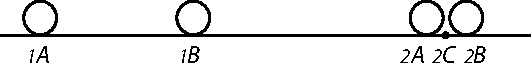
\includegraphics[width=0.475\textwidth]{gesamttex/edit_VIII,3/images/LH_37_05_146-147_d2_146r.pdf}}} \ \lbrack\textit{Fig.~2}\rbrack\ eoque casu
\textit{(2)}~si \lbrack...\rbrack\ sequitur \textit{{\scriptsize2}B} 
\textit{(a)}~, excepto uno casu quo \textit{B} ita sequitur \textit{C} ut prius attingat \textit{A}, 
quam \textit{C}, ope egredientis particulae tunc enim ordo erit 
\textit{{\scriptsize1}B{\scriptsize2}B{\scriptsize1}C{\scriptsize 2}C} 
{\protect\raisebox{-.4em}{\protect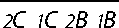
\includegraphics[width=0.11\textwidth]{gesamttex/edit_VIII,3/images/LH_37_05_146-147_d3_146r.pdf}}} \ \lbrack\textit{Fig.~3a}\rbrack\ 
\textit{(b)}~
{\protect\raisebox{-.4em}{\protect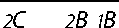
\includegraphics[width=0.11\textwidth]{gesamttex/edit_VIII,3/images/LH_37_05_146-147_d4_146r.pdf}}} \ \lbrack\textit{Fig.~3b}\rbrack\
Ideo~\textit{L}}}%
% gültiger Text:
quia si \textit{B} sequitur \textit{{\scriptsize1}C} tunc etiam \textit{{\scriptsize2}B} 
sequitur \textit{{\scriptsize2}C} et \textit{{\scriptsize1}B} sequitur \textit{{\scriptsize2}B}\lbrack:\rbrack
\pend
%
%
\vspace{1.0em} %%%%%%%%% Diagramm 4
\centerline{%
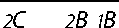
\includegraphics[width=0.145\textwidth]{%
gesamttex/edit_VIII,3/images/LH_37_05_146-147_d4_146r.pdf%
}} 
\vspace{0.5em}
\centerline{%
\lbrack\textit{Fig.~3b}\rbrack%
}
% \newpage%
\vspace{1em}
%
\newpage
\pstart\noindent
Ideo%
\edlabel{37_05_146-147_5b}
% 
erit ${\scriptstyle \textit{1}}B{\scriptstyle \textit{2}}C \sqcap {\scriptstyle \textit{1}}B{\scriptstyle \textit{2}}B + {\scriptstyle \textit{2}}B{\scriptstyle \textit{2}}C$.
%
Ergo
${\scriptstyle \textit{1}}B{\scriptstyle \textit{2}}B \sqcap \underset{\displaystyle fl\vphantom{d^2}}{{\scriptstyle \textit{1}}B{\scriptstyle \textit{2}}C} \,\leibdashv \underset{\leibdashv \displaystyle d^2}{{\scriptstyle \textit{2}}B{\scriptstyle \textit{2}}C}$.
%
Ergo
$ae + c^2 \sqcap fl + d^2$.
% 
Ergo
%
$d^2 \sqcap +ae + c^2 - fl$. 
%
et%
\rule[0cm]{0mm}{18pt}
%
$\displaystyle\frac{bf}{ae}d^2\ ({\scriptstyle \textit{2}}A{\scriptstyle \textit{2}}C) \sqcap fl + bf + \displaystyle\frac{bfc^2}{ae} - \displaystyle\frac{bffl}{ae}$.%
%
\pend
%
\pstart
%
Rursus: 
%
\rule[0cm]{0mm}{12pt}%
eodem modo, ut bis quaesivimus 
%
\edtext{\textit{{\scriptsize1}B{\scriptsize2}C},}{%
\lemma{}%
\Bfootnote{%
\textit{{\scriptsize1}B{\scriptsize2}C}, %
\textit{erg.\ L}%
}}
% =
\textit{{\scriptsize2}B{\scriptsize2}C}\lbrack,\rbrack\ ita bis quaeramus \textit{{\scriptsize1}A{\scriptsize2}C}.\ ubi quidem variationem omnium possibilium habenda est ratio. Et
% =
primum \textit{{\scriptsize1}A{\scriptsize2}C}, determinatur per \textit{{\scriptsize1}A{\scriptsize1}C} et \textit{{\scriptsize1}C{\scriptsize2}C}, corpus autem \textit{A}, et centrum potentiae\protect\index{Sachverzeichnis}{centrum potentiae} \textit{C} vel tendunt in easdem partes
% =
vel non. Si in easdem tendunt partes, rursus vel corpus \textit{A} praecedit vel sequitur centrum 
%%%%%%%%%%%%%%%%%%%%%%%%%%%%%%%%% FIN 146 R %%%%%%%%%%%%%%%%%%%%%%%
%%%%%%%%%%%%%%%%%%%%%%%%%%%%%%%%%%%%%%%%%%%%%%%%%%%%%%%%%%%%%%%%%%%
%%%%%%%%%%%%%%%%%%%%%%%%% INITIO 147 V %%%%%%%%%%%%%%%%%%%%%%%%%%%%
%%%%%%%%%%%%%%%%%%%%%%%%%%%%%%%%%%%%%%%%%%%%%%%%%%%%%%%%%%%%%%%%%%%
%
\edlabel{37_05_146-147_6a}%
\edtext{}{% NEUER ABSATZ UND VARIANTEN "potentiae"
{\xxref%
{37_05_146-147_6a}{37_05_146-147_6b}}%
\lemma{potentiae.}\Bfootnote{\lbrack147~v\textsuperscript{o}\rbrack\ \textit{(1)}~Si corpus \textit{A} sequitur centrum potentiae,
\textbar~tunc corpus \textit{B} \textit{gestr.}~\textbar\ %
vel in easdem cum \textit{A} tendit partes, vel in contrarias; si in easdem cum \textit{A} tendit partes, tunc istud \textit{B} erit illud ipsum quod supra sumsimus in easdem tendens partes et sequens centrum; si vero \textit{B} in alias atque \textit{A} tendat partes, nec proinde sequitur centrum \textit{C}, tunc ipsum \textit{A} necessario sequitur \textit{(2)}~Si~\textit{L}}}%
potentiae.
\pend
%
\pstart
\lbrack147~v\textsuperscript{o}\rbrack\ Si%
\edlabel{37_05_146-147_6b}
%
corpus \textit{A} sequitur centrum potentiae,\protect\index{Sachverzeichnis}{centrum potentiae} tunc corpus \textit{B} non sequitur, (\protect\vphantom)nam cum
%
duo
%<centr>
corpora medium habeant hoc centrum,
% =
non potest non alterum praecedere alterum sequi\protect\vphantom(). Sed hoc est contra Hypothesin; posuimus enim \textit{B} sequi. Si vero 
% =
corpus \textit{A} praecedit, tunc necessario (\textit{A}) erit inter \textit{C} et \textit{{\scriptsize2}C}, excepto uno
%
\edtext{casu\lbrack:\rbrack\ ((\textit{A}))}{\lemma{}\Bfootnote{casu\ \textbar \ cum \textit{gestr.}~\textbar\ ((\textit{A}))~\textit{L}}}
\edtext{est \lbrack inter\rbrack\ \textit{{\scriptsize2}C}}{\lemma{est}\Bfootnote{\textbar \ inter \textit{gestr., wieder gültig gemacht Hrsg.}~\textbar\ \textit{(1)}~\textit{{\scriptsize2}A} et \textit{(2)}~\textit{{\scriptsize2}C}~\textit{L}}}
%
et \textit{{\scriptsize1}C}. 
%
\edtext{Ergo duo ordines sunt: \textit{{\scriptsize1}C{\scriptsize1}A{\scriptsize2}C} et erit ${\scriptstyle \textit{2}}C{\scriptstyle \textit{1}}A \sqcap {\scriptstyle \textit{2}}C{\scriptstyle \textit{1}}C - {\scriptstyle \textit{1}}C{\scriptstyle \textit{1}}A$\lbrack;\rbrack\
%
alter \textit{{\scriptsize1}C{\scriptsize2}C{\scriptsize1}A} et erit ${\scriptstyle \textit{2}}C{\scriptstyle \textit{1}}A \sqcap -{\scriptstyle \textit{2}}C{\scriptstyle \textit{1}}C + {\scriptstyle \textit{1}}C{\scriptstyle \textit{1}}A$}{\lemma{}\Bfootnote{Ergo \lbrack...\rbrack\ $+ {\scriptstyle \textit{1}}C{\scriptstyle \textit{1}}A$ \textit{erg.}~\textit{L}}}.
%
Nimirum corpus \textit{A} 
\edtext{praecedit, et}{\lemma{praecedit,}\Bfootnote{\textit{(1)}~\textit{B} sequitur \textit{(2)}~et~\textit{L}}} 
\textit{C}.\ sequitur \textit{A}, et \textit{B} sequitur \textit{C}. 
%
Quaeritur an possit fieri ut
% =
corpus \textit{B} attingat corpus \textit{A},
%
\edtext{antequam corpus}{\lemma{antequam}\Bfootnote{\textit{(1)}~punctum \textit{(2)}~corpus~\textit{L}}}
%
\textit{A} 
%
\edtext{decurrere possit rectam}{\lemma{decurrere possit}\Bfootnote{\textit{(1)}~distantiam quanta est centri \textit{(2)}~rectam~\textit{L}}}
%
% =
quanta est \textit{{\scriptsize2}C{\scriptsize2}A}. 
%
Quod fieri potest, quia potest aliquid longe prominere ex corpore \textit{B}, ut mature attingat 
\edtext{corpus \textit{A}. Et}{\lemma{corpus \textit{A}.}\Bfootnote{\textit{(1)}~Est erg \textit{(2)}~Et~\textit{L}}} 
% =
tunc situs ipsius \textit{A} est ((\textit{A})) ponendo locum 
%
\edtext{ipsius \textit{{\scriptsize2}C} inter \textit{{\scriptsize1}C} et \textit{{\scriptsize1}A}. Denique}%
{\lemma{ipsius}%
\Bfootnote{\textit{(1)}~\textit{A} inter \textit{{\scriptsize2}C} et \textit{{\scriptsize2}A}. %
\textit{(a)}~Est ergo ${\scriptstyle \textit{2}}C{\scriptstyle \textit{1}}C - {\scriptstyle \textit{1}}C{\scriptstyle \textit{1}}A \sqcap {\scriptstyle \textit{2}}C A$
\textit{(b)}~${\scriptstyle \textit{2}}C{\scriptstyle \textit{1}}C - {\scriptstyle \textit{1}}C{\scriptstyle \textit{1}}A \sqcap {\scriptstyle \textit{2}}C{\scriptstyle \textit{1}}A$, si vero situs ipsius \textit{A}.\ est (\textit{A}) 
\textit{(2)}~\textit{{\scriptsize2}C} inter \textit{{\scriptsize1}C} et \textit{{\scriptsize1}A}. Denique~\textit{L}}}
%
si corpora \textit{A}.\textit{B} in oppositas tendant partes
% =
et sit \textit{A} illud quod in partem tendit directioni centri \textit{C}.\ contrariam, tunc rursus vel erit \textit{{\scriptsize2}C} necessario 
% =
inter \textit{A} et \textit{C}.\ nam \textit{C} est dexterius ipso \textit{A}, et \textit{{\scriptsize2}C} etiam est dexterius ipso \textit{A}, quia est in parte \textit{B}, seu inter \textit{{\scriptsize2}B} et \textit{{\scriptsize2}A}\lbrack,\rbrack\ 
% =
et \textit{{\scriptsize2}C} est sinisterius ipso \textit{C}, quia tendit dextrorsum in partes oppositas partibus \textit{C}. Ergo \textit{{\scriptsize2}C} quod est 
% =
dexterius quam \textit{A}, sinisterius quam \textit{C} est inter \textit{C} et \textit{A}.%
\pend
\newpage
\pstart
\hspace{1mm}\hspace{-1mm}% Trick, weil \edlabel nicht zu \par-Beginn sein darf
\edlabel{37_05_146-147_17a}%
Habemus ergo tres casus, unum 
%
\edlabel{37_05_146-147_7a}%
\edtext{}{% NEUER ABSATZ UND VARIANTEN – "quo"
{\xxref%
{37_05_146-147_7a}{37_05_146-147_7b}}%
\lemma{quo}\Bfootnote{\textit{(1)}~\textit{A} est \textit{(2)}~\textit{{\scriptsize1}A}~\textit{L}}}%
quo
\pend
%
\pstart
\textit{{\scriptsize1}A}%
\edlabel{37_05_146-147_7b}
%
\edlabel{37_05_146-147_15a}%	Zwecks Referenzierung in Überlieferung
est inter \textit{C} et \textit{{\scriptsize2}C}, et erit ${\scriptstyle \textit{2}}C{\scriptstyle \textit{1}}A \sqcap +{\scriptstyle \textit{2}}C{\scriptstyle \textit{1}}C - {\scriptstyle \textit{1}}C{\scriptstyle \textit{1}}A$
%
\edtext{semper cum praecedit \textit{A} per viam majorem \textit{{\scriptsize1}A} sinisterius quam
%
\edtext{\textit{{\scriptsize1}C} quia}{%
\lemma{\textit{{\scriptsize1}C}}%
\Bfootnote{%
\textit{(1)}~quia \textit{A} tendit sinistrorsum %
\textit{(2)}~quia~\textit{L}%
}}
praecedit, \textit{{\scriptsize2}C} sinisterius quam \textit{{\scriptsize1}A}, nam \textit{A} majorem facit viam quam \textit{C}.}%
{\lemma{}%
\Bfootnote{semper \lbrack...\rbrack\ quam \textit{C} \textit{erg.}~\textit{L}}} %
\pend
%
\pstart
%
\textit{{\scriptsize2}C} \dots\dots\ 
\textit{A} et \textit{{\scriptsize1}C}
\dots\dots\dots\ ${\scriptstyle \textit{2}}C{\scriptstyle \textit{1}}A \sqcap -{\scriptstyle \textit{2}}C{\scriptstyle \textit{1}}C + {\scriptstyle \textit{1}}C{\scriptstyle \textit{1}}A$
%
\edtext{nunc cum praecedit, sed per viam 
%
\edtext{minorem via centri,\protect\index{Sachverzeichnis}{via centri potentiae} \textit{{\scriptsize2}C}}{%
\lemma{minorem}%
\Bfootnote{%
\textbar \ via centri \textit{gestr. u. wieder gültig gemacht}~\textbar\ 
\textit{(1)}~si praecedit sinist
\textit{(2)}~\textit{{\scriptsize2}C}~\textit{L}%
}}
%
sinisterius quam 
\textit{{\scriptsize1}C}, si praecedit tunc enim alio \textit{B} sequente omnia tendunt ad easdem partes et
\textit{{\scriptsize1}A} sinisterius quam \textit{{\scriptsize2}C}, quando via ejus minor.}%
{\lemma{}%
\Bfootnote{nunc
\lbrack...\rbrack\ minor 
\textit{erg.}~\textit{L}}}%
\edlabel{37_05_146-147_15b} 
%
\pend
%
\pstart
%
\textit{{\scriptsize1}C} est \dots\
\textit{A} et \textit{{\scriptsize2}C} 
\phantom{et erit \dots} ${\scriptstyle \textit{2}}C{\scriptstyle \textit{1}}A 
\sqcap +{\scriptstyle \textit{2}}C{\scriptstyle \textit{1}}C + {\scriptstyle \textit{1}}C{\scriptstyle \textit{1}}A$
\edtext{nunc cum occurrit. Si occurrunt erit tunc \textit{C} dexterius quam \textit{{\scriptsize2}C}, et \textit{{\scriptsize2}C} 
dexterius quam \textit{A} (\protect\vphantom)quia dexterius quam \textit{{\scriptsize2}A}. et \textit{{\scriptsize2}A}, hoc loco dexterius quam 
\textit{{\scriptsize2}C}\protect\vphantom().}{\lemma{}\Bfootnote{nunc \lbrack...\rbrack\ \textit{{\scriptsize2}C}\protect\vphantom() \textit{erg.}~\textit{L}}} 
%
Sed hic postremus casus in \textit{A} locum habere non potest, quia 
%
\edtext{ipsi}{\lemma{}\Bfootnote{ipsi \textit{erg.}~\textit{L}}}
%
\textit{B} talem dedimus ordinem signorum. Non autem simul potest
% =
competere
%
\edtext{duobus et ostendimus per enumerationem, quia neque cum praecedit \textit{A} ipsum \textit{C}, neque cum 
occurrit locum habet.}{\lemma{duobus}\Bfootnote{\textit{(1)}~. \textbar\ Est \textit{streicht Hrsg.} \ \textbar\ 
ergo \textit{(2)}~et \lbrack...\rbrack\ habet.~\textit{L}}}
%
\pend
%
\pstart
\centering
${\scriptstyle \textit{2}}C{\scriptstyle \textit{1}}A \sqcap (\leibdashv)c^2(\leibvdash)bf$.%
\edlabel{37_05_146-147_17b}
%
\pend
%
\pstart
Superest nunc ut investigemus \textit{{\scriptsize2}C{\scriptsize1}A} per \textit{{\scriptsize1}A{\scriptsize2}A} 
et \textit{{\scriptsize2}A{\scriptsize2}C}. Nempe si \textit{A} non sequitur \textit{C} tunc vel ei occurrit,
% =
vel ipsum 
%
\edtext{praecedit, seu}{\lemma{praecedit}\Bfootnote{\textit{(1)}~. Si \textit{A} praecedit \textit{(a)}~\textit{B} \textit{(b)}~\textit{C} ex hypothesi, et semper \textit{(aa)}~\textit{A} \textit{(bb)}~\textit{{\scriptsize2}A} praecedit \textit{{\scriptsize2}C} ex natura rei \textit{(2)}~, seu~\textit{L}}}
%
\edtext{\textit{{\scriptsize2}A} semper sinisterior quam \textit{{\scriptsize2}C}, item \textit{{\scriptsize2}A} semper sinisterior quam \textit{{\scriptsize1}A},}%
{\lemma{\textit{{\scriptsize2}A} semper}%
\Bfootnote{\textit{(1)}~dexterior quam \lbrack...\rbrack\ semper dexterior quam \textit{{\scriptsize1}A},
\textit{(2)}~sinisterior \lbrack...\rbrack\ \textit{{\scriptsize1}A},~\textit{L}}} 
%
si \textit{A} praecedit \textit{C} seu in easdem 
% =
tendit partes cum \textit{C}, quod ponimus tendere sinistrorsum. Sed \textit{{\scriptsize1}A} modo dexterior quam 
\textit{{\scriptsize2}C}, modo sinisterior,
% = 
dexterior cum via  
%
\edtext{ipsius \textit{{\scriptsize1}A} (\protect\vphantom)in}{\lemma{ipsius \textit{{\scriptsize1}A} }\Bfootnote{\textit{(1)}~minor \textit{(2)}~(\protect\vphantom)in~\textit{L}}}
%
\textit{{\scriptsize2}A}\protect\vphantom() major quam via centri.\protect\index{Sachverzeichnis}{via centri potentiae} Et tunc fit ordo \textit{{\scriptsize1}A{\scriptsize2}C{\scriptsize2}A}.
a dextro
% =
ad 
%
\edtext{sinistrorsum, adeoque}{\lemma{sinistrorsum,}\Bfootnote{\textit{(1)}~quia \textit{(2)}~adeoque~\textit{L}}}
%
${\scriptstyle \textit{2}}C{\scriptstyle \textit{1}}A \sqcap -{\scriptstyle \textit{2}}C{\scriptstyle \textit{2}}A + {\scriptstyle \textit{2}}A{\scriptstyle \textit{1}}A$
%
\edtext{cum praecedit per viam majorem.}{\lemma{}\Bfootnote{cum \lbrack...\rbrack\ majorem \textit{erg.}~\textit{L}}}
%
\pend
\pstart
Vel erit \textit{{\scriptsize1}A} sinisterior quam \textit{C},
% =
\edtext{qua\lbrack ndo\rbrack}{\lemma{quam}\Bfootnote{\textit{L ändert Hrsg.}}}
%
via ab \textit{A} in \textit{{\scriptsize2}A} minor
%
\edtext{quam via a \textit{C} in}{\lemma{quam via}\Bfootnote{\textit{(1)}~ab \textit{A} in \textit{(2)}~a \textit{C} in~\textit{L}}}
%
\textit{{\scriptsize2}C}, 
%
\edtext{unde \textit{C} non praevertit}{\lemma{unde}\Bfootnote{\textit{(1)}~ergo \textit{(2)}~\textit{C} non \textit{(a)}~venit \textit{(b)}~praevertit~\textit{L}}}
%
\textit{A}, antequam
% =
veniat 
\edtext{in \textit{{\scriptsize2}A},}{\lemma{in}\Bfootnote{\textit{(1)}~\textit{B} \textit{(2)}~\textit{{\scriptsize2}A},~\textit{L}}} 
adeoque semper manet ut erat eo dexterius, ergo \textit{{\scriptsize2}C} dexterius eo casu quam \textit{A},
% =
et erit ordo: \textit{{\scriptsize2}C{\scriptsize1}A{\scriptsize2}A} et aequatio: ${\scriptstyle \textit{2}}C{\scriptstyle \textit{1}}A \sqcap +{\scriptstyle \textit{2}}C{\scriptstyle \textit{2}}A - {\scriptstyle \textit{2}}A{\scriptstyle \textit{1}}A$ cum praecedit sed per viam minorem.
% =
\pend
\newpage
\pstart Denique cum occurit \textit{A} ipsi \textit{C}, tunc quidem \textit{{\scriptsize2}A} erit semper sinisterior quam 
%
\edtext{\textit{{\scriptsize2}C} ex natura rei. Sed et \textit{{\scriptsize2}A}}{\lemma{\textit{{\scriptsize2}C}}\Bfootnote{\textit{(1)}~et erit \textit{(2)}~ex natura rei. Sed
\textbar\ et \textit{erg.}~\textbar\ %
\textit{{\scriptsize2}A}~\textit{L}}}
%
dexterior etiam
% =
quam \textit{{\scriptsize1}A}, quia \textit{A}, tendit dextrorsum, ergo fiet ordo 
\edtext{a dextro}{\lemma{}\Bfootnote{a dextro \textit{erg.}~\textit{L}}} 
\textit{{\scriptsize2}C{\scriptsize2}A{\scriptsize1}A}, et fiet aequatio:
% =
${\scriptstyle \textit{2}}C{\scriptstyle \textit{1}}A \sqcap +{\scriptstyle \textit{2}}C{\scriptstyle \textit{2}}A\, +\, $%
%
%
\edlabel{37_05_146-147_8a}%
\edtext{}{% NEUER ABSATZ UND VARIANTEN
{\xxref%
{37_05_146-147_8a}{37_05_146-147_8b}}%
\lemma{\textit{{\scriptsize2}A{\scriptsize1}A}.}\Bfootnote{\textit{(1)}~Ergo erit  \textit{(2)}~Ergo ut omnia colligamus,~\textit{L}}}%
\textit{{\scriptsize2}A{\scriptsize1}A}.
\pend
%
\pstart
Ergo ut omnia colligamus,%
\edlabel{37_05_146-147_8b}
%
erit in casu occursus\protect\index{Sachverzeichnis}{occursus} ${\scriptstyle \textit{2}}C{\scriptstyle \textit{1}}A \sqcap +{\scriptstyle \textit{2}}C{\scriptstyle \textit{2}}A + {\scriptstyle \textit{2}}A{\scriptstyle \textit{1}}A \sqcap -{\scriptstyle \textit{2}}C{\scriptstyle \textit{1}}C+{\scriptstyle \textit{1}}C{\scriptstyle \textit{1}}A$ 
%
%
\pend
%
\pstart\noindent
at in casu praecedentiae\protect\index{Sachverzeichnis}{praecedentia} per viam majorem via centri erit
%
\pend\pstart
\raggedleft
${\scriptstyle \textit{2}}C{\scriptstyle \textit{1}}A \sqcap -{\scriptstyle \textit{2}}C{\scriptstyle \textit{2}}A + {\scriptstyle \textit{2}}A{\scriptstyle \textit{1}}A \sqcap +{\scriptstyle \textit{2}}C{\scriptstyle \textit{1}}C - {\scriptstyle \textit{1}}C{\scriptstyle \textit{1}}A$
%
\pend\pstart
\newlength{\incasupraecedentiae}
\newlength{\majoremviacentri}
\settowidth{\incasupraecedentiae}{ut in casu praecedentiae per viam}
\settowidth{\majoremviacentri}{majorem via centri erit}
\noindent\parbox[b][0 pt][b]{\incasupraecedentiae}{$\dotfill$}
\parbox[b][0 pt][b]{\majoremviacentri}{minorem $\dotfill$} 
%
\pend\pstart
\raggedleft
${\scriptstyle \textit{2}}C{\scriptstyle \textit{1}}A \sqcap +{\scriptstyle \textit{2}}C{\scriptstyle \textit{2}}A - {\scriptstyle \textit{2}}A{\scriptstyle \textit{1}}A \sqcap -{\scriptstyle \textit{2}}C{\scriptstyle \textit{1}}C + {\scriptstyle \textit{1}}C{\scriptstyle \textit{1}}A$.
%
\pend\pstart
\noindent 
%
Ergo%
\rule[0cm]{0mm}{14pt} 
%
\edlabel{37_05_146-147_13a}%
\edtext{}{% A-Footnote
{\xxref%
{37_05_146-147_13a}{37_05_146-147_13b}}%
\lemma{}%
\Afootnote{%
\textit{Unterhalb \textup{Ergo \textit{{\scriptsize 2}C{\scriptsize 1}A} \lbrack...\rbrack\ Seu \textit{{\scriptsize 2}C{\scriptsize 1}A}}:}\enskip
(\protect\vphantom)Si non potuissent omnia tam in una quam in alia aequatione ad tres reduci casus, sed in una fuissent aliae faciendae subdivisiones quam in alia nonnullis licet coincidentibus, tunc ducendo divisionem in divisionem potuissent fieri tot casus quot minimae species. NB.\lbrack\protect\vphantom()\rbrack%
}}%
%
${\scriptstyle \textit{2}}C{\scriptstyle \textit{1}}A \sqcap \underset{\displaystyle +}{\underset{\displaystyle -}{+}}{\scriptstyle \textit{2}}C{\scriptstyle \textit{2}}A \underset{\displaystyle -}{\underset{\displaystyle +}{+}} {\scriptstyle \textit{2}}A{\scriptstyle \textit{1}}A \sqcap \underset{\displaystyle -}{\underset{\displaystyle +}{-}} {\scriptstyle \textit{2}}C{\scriptstyle \textit{1}}C \underset{\displaystyle +}{\underset{\displaystyle -}{+}} {\scriptstyle \textit{1}}C{\scriptstyle \textit{1}}A$. 
%
Seu
%
${\scriptstyle \textit{2}}C{\scriptstyle \textit{1}}A%
\edlabel{37_05_146-147_13b}
\sqcap \mathop{\pmH} \underset{\displaystyle \frac{bf}{ae}d^2}{{\scriptstyle \textit{2}}C{\scriptstyle \textit{2}}A} \mathop{\pmG} \underset{\vphantom{\dfrac{f}{e}}\displaystyle el}{{\scriptstyle \textit{2}}A{\scriptstyle \textit{1}}A} \sqcap \mathop{\pmB} \underset{\vphantom{\dfrac{f}{e}}\displaystyle c^2}{{\scriptstyle \textit{2}}C{\scriptstyle \textit{1}}C} \mathop{\pmH} \underset{\vphantom{\dfrac{f}{e}}\displaystyle bf}{{\scriptstyle \textit{1}}C{\scriptstyle \textit{1}}A}$.
%
\pend
%
\pstart
Ergo 
\rule[0cm]{0mm}{18pt}%
$\displaystyle\frac{bf}{ae}d^2 \sqcap -c^2\,\ovalbox{+\textit{bf}}\ \pmD el$ et supra erat idem: $\sqcap\ \ovalbox{$+bf$} + \displaystyle\frac{bfc^2}{ae} - \displaystyle\frac{bffl}{ae}$.
\pend 
\pstart\noindent
Fietque: $c^2ae + c^2bf \sqcap + bffl \,\pmD\, ae^2l$.\ et $c^2\, \sqcap\,$%
%
\edtext{$\displaystyle\frac{bffl \,\pmD\, aeel}{ae+bf}$. Jam}{\lemma{$\displaystyle\frac{bffl \,\pmD\, aeel}{ae+bf}$}\Bfootnote{\textit{(1)}~et quia idem $\sqcap\, bmml \,\pmD\, a$ \textit{(2)}~. Jam~\textit{L}}}
% 
examinandum quae sint signa in omnibus tribus casibus post
%
\edtext{concursum.\protect\index{Sachverzeichnis}{concursus} Idem}{\lemma{concursum.}\Bfootnote{\textit{(1)}~Accedit enim casus divergentiae quem in prioribus non consideravimus. Itaque res altius repetenda atque universalius tractanda est. \textit{(2)}~Idem~\textit{L}}}
%
\edtext{$c^2 \sqcap \displaystyle\frac{(+)bmml((+))aiil}{ae+bf}$. Quia}{\lemma{$c^2 \sqcap \displaystyle\frac{(+)bmml((+))aiil}{ae+bf}$.}\Bfootnote{\textit{(1)}~Erunt ergo \textit{(2)}~Quia~\textit{L}}} 
% =
eadem semper via centri gravitatis,\protect\index{Sachverzeichnis}{via centri gravitatis} tantum signa quaerenda sunt.
%
\edlabel{37_05_146-147_18a}%
Interim
%
\rule[0cm]{0mm}{12pt}%
$bf^2 \pmD ae^2 \sqcap (+)bm^2 ((+)) ai^2$. 
Seu $(+)bm^2 - bf^2 \sqcap \pmD ae^2 ((-)) ai^2$. 
%
\rule[0cm]{0mm}{18pt}%
Seu $\displaystyle\frac{a}{b} \sqcap \displaystyle\frac{(+)m^2 - f^2}{\pmD e^2 ((-)) i^2} \sqcap \displaystyle\frac{m-f}{e-i}$. 
Ex priore aequatione $\displaystyle\frac{a}{b} \sqcap \displaystyle\frac{m-f}{e-i}$.\ seu $ae-ai \sqcap bm - bf$.\ erit 
%
\rule[0cm]{0mm}{16pt}%
$m \sqcap \displaystyle\frac{ae-ai}{b} + f$ 
%
seu $m \sqcap$ \makebox[1.0\textwidth][s]{$\displaystyle\frac{a}{b}\;\overline{e-i}+f$.\ 
et erit 
%
$(+) bm^2 \sqcap (+) \displaystyle\frac{\cancel{b}a^2}{b^{\cancel{2}}}\;\overline{e^2-2ei+i^2}\;(+)bf^2(+) \cancel{b} \displaystyle\frac{2af}{\cancel{b}}\;\overline{e-i}$. Et $(+)bm^2 - bf^2 \sqcap$}
\pend
\newpage
\pstart
\noindent $(+) \displaystyle\frac{a^2}{b}\; \overline{e^2-2ei+i^2}\;(+)bf^2(+)2af\;\overline{e-i} \sqcap \pmD ae^2 ((-)) ai^2$,
%
et habebitur aequatio explicans valorem ipsius \textit{f}, ubi 
%
\rule[0cm]{0mm}{10pt}%
posito esse $(+) \sqcap +$ aequatio reddetur multo
% =
simplicior, simplicissima autem si 
%
\rule[0cm]{0mm}{16pt}%
praeterea $\pmD$ valeat $+$, et $((-))$ valeat $-$\lbrack,\rbrack\ tunc enim fiet $\displaystyle\frac{m+f}{e+i} \sqcap \displaystyle\frac{a}{b}$ quod tamen
% =
semper locum non habet. 
%
\rule[0cm]{0mm}{10pt}Semper autem videtur $((+))$ significare $+$, seu $+$ praefigi ipsi \textit{aiil} uti praefixum est plus ipsi \textit{bffl}, in 
% =
calculo viae centri,\protect\index{Sachverzeichnis}{via centri potentiae} quia ut ab \textit{{\scriptsize1}B} ad \textit{{\scriptsize2}B} eundo et ab \textit{{\scriptsize1}C} ad \textit{{\scriptsize2}C}, \textit{B} sequitur \textit{C}, ita eundo a \textit{{\scriptsize3}B} ad \textit{{\scriptsize2}B} vel a \textit{{\scriptsize3}C} ad \textit{{\scriptsize2}C}.\ semper \textit{A} sequitur \textit{C}.
% =
%
\pend
%
\pstart
Ergo 
%
\rule[0cm]{0mm}{16pt}%
$\displaystyle\frac{a}{b} \sqcap %
%
\edtext{\displaystyle\frac{(+)m^2-f^2}{\pmD e^2-i^2} \sqcap \displaystyle\frac{m-f}{e-i}$.}{%
\lemma{$\displaystyle\frac{(+)m^2-f^2}{\pmD e^2-i^2}$}%
\Bfootnote{%
\textit{(1)}~. Hinc si $(+) \sqcap \pmD $ %
\textit{(2)}~$ \sqcap \displaystyle\frac{m-f}{e-i}$.~\textit{L}}}%
\edlabel{37_05_146-147_18b}
\pend
% =
%%%%%%%%%%%%%%%%%%%%%%%%%%%%%%% FIN 147 v %%%%%%%%%%%%%%%%%%%%%%%%%%%%%%%%%%%%%%
%%%%%%%%%%%%%%%%%%%%%%%%%%%%%%%%%%%%%%%%%%%%%%%%%%%%%%%%%%%%%%%%%%%%%%%%%%%%%%%%
%%%%%%%%%%%%%%%%%%%%%%%%%%%%%%%INITIO 147 R%%%%%%%%%%%%%%%%%%%%%%%%%%%%%%%%%%%%%
%
%%
\vspace{1.0em}	% müsste normalerweise 0.5em sein, aber der Bruch in der vorigen Zeile verschlingt etwas von der nachfolgenden Zeilenhöhe; wird durch 1.0em kompensiert
\pstart
\noindent
\lbrack%
\textit{Nachfolgender Text bis S.~\refpassage{37_05_146-147_20}{37_05_146-147_20}: erster Anlauf zu S.~\refpassage{37_05_146-147_19}{37_05_146-147_19}ff.}\rbrack 
\pend
\vspace{0.5em}
%
\pstart 
\noindent
\edtext{\lbrack147~r\textsuperscript{o}\rbrack\ %	B-Fn
\edlabel{37_05_146-147_14a}%		
\edtext{}{% überkreuzte C-Fn (Fehler in Rechnung)
{\xxref%
{37_05_146-147_14a}{37_05_146-147_14b}}%
\lemma{$\displaystyle\frac{a}{b} \sqcap \displaystyle\frac{e-i}{m-f}\sqcap \displaystyle\frac{\pmD\; e^2-i^2}{(+)m^2-f^2}$}%
\Cfootnote{%
Die linke Seite der Gleichung lautet richtig: $\dfrac{b}{a}$. Der Fehler wirkt sich auf sämtliche Rechnungen im folgenden Absatz aus.%
}}%
$\displaystyle\frac{a}{b}\; \sqcap$}{\lemma{\lbrack147~r\textsuperscript{o}\rbrack}\Bfootnote{\textit{(1)}~Si $e+i\, \groesser$ quam $f+m$ et \textit{b} maj \textit{(2)}~$\displaystyle\frac{a}{b}\sqcap$~\textit{L}}}
%
$\displaystyle\frac{e-i}{m-f}\sqcap \displaystyle\frac{\pmD\; e^2-i^2}{(+)m^2-f^2}$.%
\edlabel{37_05_146-147_14b}
%
\pend \pstart 
Ponamus 
%
\rule[0cm]{0mm}{10pt}%
\textit{a} esse $\groesser\, b$. Erit $e-i\, \groesser\, m-f$. Quod si jam et $e+i\, \groesser\, m+f$
% =
erit et $+e^2-i^2\, \groesser\, m^2-f^2$. At $\pmD\, e^2-i^2$ etiam $\groesser\, (+)m^2-f^2$. Ergo si $\pmD$ est $+$
% =
erit $e^2-i^2\, \groesser\, m^2-f^2$, 
%
\edtext{itemque $\groesser\, (+)m^2-f^2$. Ergo}{\lemma{itemque $\groesser\, (+)m^2-f^2$.}\Bfootnote{\textit{(1)}~Quod fieri potest \textit{(2)}~Ergo~\textit{L}}}
%
si $(+)$ est $-$ erit
% =
$e^2-i^2\, \groesser\, m^2-f^2$ et $-m^2-f^2$.\ quod fieri potest, seu $2e^2-2i^2\, \groesser\, -2f^2$, seu $e^2\, \groesser\, i^2-f^2$
% =
seu
%
\edtext{$e^2+f^2\, \groesser\, i^2$.\ quod}{\lemma{$e^2+f^2\, \groesser\, i^2$.}\Bfootnote{\textit{(1)}~ergo $e\, \groesser\, i$ \textit{(2)}~quod~\textit{L}}}
% 
possibile. Sed non ut sit $\pmD\; \sqcap -$. In hoc casu
% =
fieret enim $e^2 - i^2\, \groesser\, +m^2 - f^2$, et $-e^2-i^2\, \groesser\, 
%
\edtext{(+)m^2-f^2$. Ergo \textit{m}}{\lemma{$(+)m^2-f^2$.}\Bfootnote{\textit{(1)}~Ergo \textit{(a)}~\textit{m} \textit{(b)}~$(+)$  necessario $+$. \textit{(2)}~Ergo si $a\, \groesser$ \textit{(3)}~Ergo \textit{m}~\textit{L}}}
%
non potest 
%
\edtext{esse $+$. Sit enim}{\lemma{esse $+$.}%
\Bfootnote{%
\textit{(1)}~Ergo si $a\, \groesser\, b$ et $e+i\, \groesser\, m+f$ et %
\textbar\ $\pmD$ est %
\textit{(a)}~$+$ %
\textit{(b)}~$-$ \textit{streicht Hrsg.}~\textbar\ %
tunc etiam $(+)$ est %
\textit{(aa)}~$+$ %
\textit{(bb)}~$-$ %
\textit{(2)}~Sit enim~\textit{L}}}
%
$-e^2-i^2\, \groesser\, +m^2-f^2$.
%
Ergo $f^2\, \groesser\, m^2+e^2+i^2$.
% =
Ergo $f^2-m^2\, \groesser\, e^2+i^2$. Ergo 
\edtext{et $f^2-m^2\, \groesser\, e^2-i^2$.}{\lemma{et}\Bfootnote{\textit{(1)}~$f^2$ erit $\kleiner$
\textbar\ ergo et \textit{streicht Hrsg.}~\textbar\  \textit{(2)}~$f^2-m^2\, \groesser\, e^2-i^2$~\textit{L}}}
Dividatur majus per minus
% =
seu per $m+f$, et minus $e^2-i^2$ per majus \makebox[1.0\textwidth][s]{$e+i$ (positis omnibus in integris) manebit 
% =
$f-m\, \groesser\, e-i$. Ergo $f-m\, \groesser\, m-f$ seu $f\, \groesser\, m$.}
\pend
\newpage
\pstart
\noindent Ergo hoc casu rursus signa eadem,
% =
seu si $a\, \groesser\, b$. et $e+i\, \groesser\, m+f$. et $f\, \groesser\, m$, adeoque et $e\, \groesser\, i$ et $\pmD\,\sqcap -$ erit et $(+)\sqcap -$.
\pend 
\pstart
Video jam errorum fontes quod pro \textit{e} substitui
% =
indifferenter \textit{i}, et pro \textit{f}, substitui 
%
\edtext{\textit{m}, quod}{\lemma{\textit{m}, }\Bfootnote{\textit{(1)}~cum autem \textit{(2)}~quod~\textit{L}}}
%
fieri potest in expressione celeritatum, sed fieri non potest
% =
in expressione partium in
%
\edtext{quas distantia corporum\protect\index{Sachverzeichnis}{distantia corporum} per}{\lemma{quas}\Bfootnote{%
\textit{(1)}~centrum gravitatis secatur %
\textit{(2)}~distantia corporum
\textit{(a)}~seca \textit{(b)}~per
\textit{L}}}
%
centrum potentiae\protect\index{Sachverzeichnis}{centrum potentiae} secatur. Calculus ergo novus cautissime ineundus.\edlabel{37_05_146-147_20}
\pend 
%
\vspace{0.5em}
\pstart
\noindent
\lbrack%
\textit{Zweiter Anlauf:}\rbrack 
\pend
\vspace{0.5em}
%
\pstart\noindent
$\astrosun\edlabel{37_05_146-147_19} %Referenz
%
\displaystyle\frac{a}{b}\sqcap \displaystyle\frac{(+)m^2-f^2}{\pmD\; e^2-i^2}\sqcap\displaystyle\frac{m-f}{e-i}$
%
\edtext{ut ostendimus pagina versa.\edlabel{37_05_146-147_2a}}{%
\lemma{ut ostendimus pagina versa}%
\Cfootnote{%
Siehe S.~\refpassage{37_05_146-147_18b}{37_05_146-147_18b}.}}%
%
\edtext{}{{\xxref{37_05_146-147_2a}{37_05_146-147_2b}}\lemma{versa.}\Bfootnote{\textit{(1)}~Ergo $(+)\sqcap \pmD$ \textit{(2)}~Nam~\textit{L}}}
\pend\pstart
Nam\edlabel{37_05_146-147_2b}
%
ponamus $(+)$ esse $+$; et $\pmD$ esse $-$. Fiet $\displaystyle\frac{+m^2-f^2}{-e^2-i^2}\sqcap\displaystyle\frac{m-f}{e-i}$.
%
Ergo 
%
\edtext{(aut $m\sqcap f$ unde et $e \sqcap i$ quo casu et $a\sqcap b$ aut)}{\lemma{}%
\Bfootnote{(\protect\vphantom)aut $m\sqcap f$ \textbar\ unde et $e \sqcap i$ quo casu et $a\sqcap b$  \textit{erg.}~\textbar\ aut\protect\vphantom()~\textit{erg.}~\textit{L}}}
%
dividendo utrobique
% =
per $m-f$ fiet:
%
\edtext{$m+f \sqcap \displaystyle\frac{-e^2-i^2}{e-i}$ quod est}{%
\lemma{$m+f \sqcap \displaystyle\frac{-e^2-i^2}{e-i}$}%
\Bfootnote{\textit{(1)}~\textbar\ $\sqcap$ \textit{streicht Hrsg.} \textbar\  $\displaystyle\frac{+e^2-i^2}{e-i} - \displaystyle\frac{2e^2}{e-i} \sqcap e+i - \displaystyle\frac{2e^2}{e-i}$. Est autem \textit{e} major \textit{i}, si \textit{(2)}~quod \textit{(a)}~si $(+) \sqcap -$ erit \textit{(b)}~\textbar\ quod \textit{erg., streicht Hrsg.}~\textbar\ est~\textit{L}}}
% 
\rule[0cm]{0mm}{10pt}
absurdum posito \textit{e} esse majus quam \textit{i}, foret enim
%
\edtext{quantitas negativa\protect\index{Sachverzeichnis}{quantitas negativa}}{\lemma{quantitas}\Bfootnote{\textit{(1)}~imaginaria \textit{(2)}~negativa~\textit{L}}}
%
\edtext{aequalis affirmativae\protect\index{Sachverzeichnis}{quantitas affirmativa}}{\lemma{aequalis}\Bfootnote{\textit{(1)}~verae \textit{(2)}~affirmativae~\textit{L}}}.
%
Ergo, si $e\,\groesser\, i$ vel $m\,\groesser\, f$, tunc 
%
\rule[0cm]{0mm}{12pt}%
semper posito $(+)$ esse $+$ etiam $\pmD$ erit $+$
% =
et vicissim posito $\pmD$ esse $-$, eo in casu etiam $(+)$ erit $-$. 
\pend \pstart
Sit jam $(+)\sqcap -$ et $\pmD\,\sqcap +$ tunc fiet
\rule[0cm]{0mm}{16pt}%
$\displaystyle\frac{-m^2-f^2}{+e^2-i^2}\sqcap \displaystyle\frac{m-f}{e-i}$,
seu
%
\edtext{(nisi $e\sqcap i$ vel $m\sqcap f$) erit}{\lemma{}\Bfootnote{(nisi $e\sqcap i$ vel $m\sqcap f$) erit \textit{erg.}~\textit{L}}}
%
$e+i \sqcap \displaystyle\frac{-m^2-f^2}{m-f}$, quod
% =
rursus
%
\edtext{absurdum nisi}{\lemma{absurdum}\Bfootnote{\textit{(1)}~si \textit{(2)}~nisi~\textit{L}}}
%
\textit{f} sit major quam \textit{m}. Ergo generaliter concludi potest, 
%
\rule[0cm]{0mm}{10pt}%
\edtext{\;\textso{si $m\ \groesser\; f$},}{\lemma{\textso{si $m\ \groesser f$}}\Cfootnote{Doppelt unterstrichen.}} 
\edtext{seu $e\, \groesser\, i$}{\lemma{seu}\Bfootnote{\textit{(1)}~$e\, \kleiner\, i$ \textit{(2)}~$e\, \groesser\, i$~\textit{L}}}
% =
id est, si celeritas corporis ejus quod centrum potentiae\protect\index{Sachverzeichnis}{centrum potentiae} sequitur, augetur, alterius vero minuitur, tunc \edtext{\textso{signa}}{\lemma{\textso{signa}}\Cfootnote{Doppelt unterstrichen.}}
% =
$(+)$ et $\pmD$ \edtext{\textso{eadem sunt.}}{\lemma{\textso{eadem sunt}}\Cfootnote{Doppelt unterstrichen.}} 
%
\pend
%
\pstart
Videndum an eadem ratione concludi possit, diversa haec signa esse, 
% = 
quoties con- \makebox[1.0\textwidth][s]{trarium est in 
%
\edtext{celeritatibus. Ponamus}{\lemma{celeritatibus.}\Bfootnote{\textit{(1)}~Id vero manifestum est \textit{(2)}~Nam resumta aequatione \textit{(3)}~Ponamus~\textit{L}}}
%
signa esse eadem, et quidem 
%
\edtext{primo}{\lemma{}\Bfootnote{primo \textit{erg.}~\textit{L}}}
%
utrobique $+$,}
\pend
\newpage
\pstart
\noindent fiet: 
%
\rule[0cm]{0mm}{16pt}%
$\displaystyle\frac{+m^2-f^2}{+e^2-i^2}\sqcap \displaystyle\frac{m-f}{e-i}$. Ergo $\displaystyle\frac{m+f}{e+i}\sqcap 1$. 
%
\edtext{(vel $m-f \sqcap 0$ vel $e-i \sqcap 0$)}{\lemma{}\Bfootnote{(vel $m-f \sqcap 0$ vel $e-i \sqcap 0$) \textit{erg.}~\textit{L}}}
%
seu $m+f \sqcap e+i$
% =
seu $e-f \sqcap m-i$. 
\rule[0cm]{0mm}{10pt}%
Ergo si $e\, \groesser$ quam \textit{f} etiam $m\, \groesser\, i$. Unde 
%
\edtext{$m \sqcap e+i-f$ et supra}
{\lemma{$m \sqcap e+i-f$}\Bfootnote{%
\textit{(1)}~\textbar\ $\sqcap$ \textit{streicht Hrsg.}~\textbar\
$\displaystyle\frac{ae-ai+fm}{b}$
\textit{(2)}~et 
\textit{(a)}~$\displaystyle\frac{be+bi-fb}{f} \sqcap m \sqcap e+i-f$. Ergo 
\textit{(b)}~supra~\textit{L}}}
%
$ae-ai \sqcap bm-bf$ et $m \sqcap \displaystyle\frac{ae-ai+bf}{b}\sqcap e+i-f$.
% =
Ergo fiet $ae-ai \sqcap be+bi-2bf$. Et $i \sqcap \displaystyle\frac{ae-be+2bf}{a+b}$ et $m \sqcap e+\displaystyle\frac{ae-be+2bf}{a+b}-f,\sqcap \displaystyle\frac{ae\,\ovalbox{$+be$}+ae\,\ovalbox{$-be$}+2bf-af-bf}{a+b}$
% =
seu 
\edtext{$m\ \sqcap\ \displaystyle\frac{2ae-af+bf}{a+b}$. et}{\lemma{$m\ \sqcap\ \displaystyle\frac{2ae-af+bf}{a+b}$}\Bfootnote{\textit{(1)}~$m-f$ $\sqcap$ \textit{(2)}~et~\textit{L}}}
$f\ \sqcap\ \displaystyle\frac{af+bf}{a+b}$.
%
\rule[0cm]{0mm}{18pt}%
Ergo $m-f\ \sqcap\ \displaystyle\frac{2ae-af+bf-af-bf}{a+b}$
% =
seu $m-f\ \sqcap\ \displaystyle\frac{2ae-2af}{a+b}$.\ et $e-i\ \sqcap\ \displaystyle\frac{2be-2bf}{a+b}$. 
%
\rule[0cm]{0mm}{16pt}%				
\edtext{Ubi ut sciamus an \textit{m} sit $\groesser\, f$, scire oportet an sit}{\lemma{Ubi}\Bfootnote{\lbrack...\rbrack\ an sit \textit{erg.}~\textit{L}}}  
%
$e\; \groesser\, f$. 
Ergo 
%
\edtext{\;\textso{si signa sunt $+$ et $m\ \groesser\, f$ etiam erit $e\ \groesser\, f$ et $m\ \groesser\, i$.}%
}{\lemma{\textso{si signa }\lbrack...\rbrack\textso{ $m\ \groesser\, i$}}%
\Cfootnote{Doppelt unterstrichen.}}%
% =
\pend 
%
\pstart
\edtext{\textso{Si $m\ \groesser\, f$ signa sunt eadem}.}{\lemma{\textso{Si} \lbrack...\rbrack\  \textso{eadem.}}\Cfootnote{Doppelt unterstrichen.}} 
%
Ergo si signa non sunt eadem \textit{m} non est majus 
% =
%
\edtext{quam \textit{f}. Omnis}{\lemma{quam \textit{f}.}\Bfootnote{\textit{(1)}~In omni casu in quo \textit{(2)}~Omnis~\textit{L}}}
%
casus in quo 
\edtext{$m\, \groesser\, f$. est}{\lemma{$m\, \groesser\, f$.}\Bfootnote{\textit{(1)}~habet signa eadem \textit{(2)}~est~\textit{L}}}
casus habens signa eadem. Eadem id est non
% =
diversa.
%
Ergo omnis casus in quo
%
\edtext{$m\, \groesser$ \textit{f}}{%
\lemma{}%
\Bfootnote{%
$m\, \groesser$ \textbar\ majus \textit{streicht Hrsg.}~\textbar\ \textit{f}~\textit{L}}}
%
non est casus habens signa diversa. Ergo conversione
% =
simplici: Omnis casus habens signa diversa non est casus in quo
%
\edtext{$m\; \groesser$}{\lemma{\textit{m}}\Bfootnote{\textit{(1)}~majus \textit{(2)}~$\groesser$~\textit{L}}}
% 
\textit{f}. Sed quando \textit{m} non est $\groesser\, f$ tunc $m\, \kleiner\, f$.
%
(Nam ubi aequale tunc potest sumi pro alterutro errore\protect\index{Sachverzeichnis}{error infinite parvus} posito infinite parvo.) 
%
Ergo omnis casus habens signa diversa est casus
% =
in quo \textit{m} minus \textit{f}. Conclusimus ergo: 1.\ Quando $m\, \groesser\, f$ signa eadem. 
%
\edtext{2.\ cum}{%
\lemma{}%
\Bfootnote{%
2.\ \textbar\ Ergo \textit{gestr.}~\textbar\ cum~\textit{L}%
}}
%
signa diversa $m\, \kleiner\, f$. Conversione
% =
per
%
\edtext{contrapositionem\protect\index{Sachverzeichnis}{conversio per contrapositionem} si}{%
\lemma{}%
\Bfootnote{%
contrapositionem \textbar\ (\protect\vphantom) \textit{streicht Hrsg.}~\textbar\ %
si~\textit{L}%
}}
%
$m\, \groesser\, f$ signa sunt simul eadem.
%
\edtext{Si signa sunt $+$}{\lemma{Si}\Bfootnote{signa sunt \textit{(1)}~eadem \textit{(2)}~$+$~\textit{L}}}
%
et $m\, \groesser\, f$ etiam $e\, \groesser\, f$. Ergo 
%
\edlabel{37_05_146-147_16a}%
\edtext{}{% C-Footnote
{\xxref%
{37_05_146-147_16a}{37_05_146-147_16b}}%
\lemma{\textso{si signa sunt $+$ etiam $e\ \groesser\, f$}}\Cfootnote{Doppelt unterstrichen.}}%
\textso{si signa}
%
\edtext{\textso{sunt $+$}}{%
\lemma{\textso{sunt}}%
\Bfootnote{%
\textit{(1)}~\textso{eadem} \textit{(2)}~$+$~\textit{L}%
}}
%
\textso{etiam}
%
\edtext{\;\textso{$e\ \groesser\, f$.}\edlabel{37_05_146-147_16b} (\protect\vphantom)Notabile}{\lemma{$e\, \groesser\, f$.}\Bfootnote{\textit{(1)}~(\protect\vphantom)Notabilis \textit{(2)}~(\protect\vphantom)Notabile~\textit{L}}}
consequentiae logicae\protect\index{Sachverzeichnis}{consequentia logica} exemplum\protect\vphantom().\protect\index{Sachverzeichnis}{exemplum notabile consequentiae logicae} Ergo si $e\, \kleiner\, f$
%
\edtext{signa non}{\lemma{signa}\Bfootnote{\textit{(1)}~sunt diversa \textit{(2)}~non~\textit{L}}}
%
sunt $+$ utrobique.
\pend
\newpage
%
%
%%%%%%%%%%%%%%%%%%%%%%%%%%%%%%%%%%%%%%%%%%%%%%%%%%%%%%%%%%%%%%%%%%%
%%%%%%%%%%%%%%%%%%%%%%%%%%%%%%%%% FIN 147 R %%%%%%%%%%%%%%%%%%%%%%%
\pstart
\lbrack146~v\textsuperscript{o}\rbrack\
$\displaystyle\frac{\pmD\; e^2 - i^2}{(+) m^2 - f^2} \sqcap \displaystyle\frac{e-i}{m-f}$.
Si $\pmD$ est $+$ tunc fiet $\displaystyle\frac{(+) m^2 - f^2}{+e+i} \sqcap +m-f$.
%
Multiplicando illinc per $e+i$, hic per $m+f$, 
%
\rule[0cm]{0mm}{10pt}%
fiet illic $(+)m^2 - f^2$, hic $+m^2-f^2$. 
% =
\edtext{Hinc sequitur si $\pmD$ est}{\lemma{Hinc}\Bfootnote{\textit{(1)}~multiplicando \textit{(2)}~sequitur si 
\textit{(a)}~$e+i \sqcap m+f$ necessario et
\textit{(b)}~$\pmD$ est
\textit{L}}}
%
$+$ et $e+i \sqcap m+f$ tunc necessario
% =
et $(+)$ est $+$. Et si $\pmD$ est $+$ et $(+)$ est $+$
%
\edtext{erit $e+i \sqcap m+f$. Impossibile}{\lemma{erit $e+i \sqcap m+f$.}\Bfootnote{\textit{(1)}~Rursus si \textit{(a)}~\textit{e} \textit{(b)}~\textit{e} \textit{(2)}~Si vero $e+i\, \groesser$ quam $m+f$ \textit{(3)}~Impossibile~\textit{L}}}
%
est porro eo casu quo $\pmD$ est $+$ esse $e+i\, \groesser$ quam $m+f$ quia impossibile est esse $(+)m^2-f^2\, \groesser\, +m^2-f^2$
% =
seu esse 
%
\edtext{$(+)m^2\, \groesser\, +m^2$. Si}{\lemma{$(+)m^2\, \groesser\, +m^2$.}\Bfootnote{\textit{(1)}~Ergo \textit{(2)}~Si~\textit{L}}}
% 
vero $e+i\ \kleiner$ quam 
\edtext{$m+f$ et}{\lemma{$m+f$}\Bfootnote{\textit{(1)}~tunc \textit{(2)}~et~\textit{L}}}
$\pmD$ est $+$ tunc necessario $(+)$ est $-$.
% =
Si $\pmD$ est $-$ tunc fiet: $\displaystyle\frac{-e^2-i^2}{(+)m^2-f^2}\ \sqcap\ \displaystyle\frac{e-i}{m-f}$, ubi si  
\edtext{$m\, \groesser\, f$ necessario}{\lemma{$m\, \groesser\, f$}\Bfootnote{\textbar \ vel aequalis \textit{erg.~u.~gestr.}~\textbar\ necessario~\textit{L}}}
\textit{m} est $-$.
% =
Si vero \textit{m}   
%
est minor
%  
quam \textit{f}, et \textit{m} est $+$, tunc fiet
%
\rule[0cm]{0mm}{16pt}%
$\displaystyle\frac{-e^2-i^2}{m+f}\ \sqcap\ e-i$. Et 
% =
\edtext{multiplicando illinc per $m+f$ hic per $e+i$, fiet illinc $-e^2-i^2$,}{\lemma{multiplicando}\Bfootnote{\textit{(1)}~hic per $m+f$ illinc
\textit{(2)}~illinc per $m+f$ hic per $e+i$, fiet
\textit{(a)}~$-e^2-i^2$ illinc, \textit{(b)}~illinc $-e^2-i^2$,~\textit{L}}}
%
hic $e^2-i^2$,
\rule[0cm]{0mm}{10pt}%
\edtext{ergo non possunt}{\lemma{ergo}\Bfootnote{\textit{(1)}~necessario \textit{(2)}~non possunt~\textit{L}}}
%
esse $e+i$ et $m+f$
% =
\edtext{aequales, imo}{\lemma{aequales,}\Bfootnote{\textit{(1)}~nec \textit{(2)}~imo~\textit{L}}}
%
non potest non esse $+e+i$ major quam $m+f$. 
%
\edlabel{37_05_146-147_22a}%
Ergo 
\edtext{si $\pmD$ est}{\lemma{si $\pmD$}\Bfootnote{\textit{(1)}~esset \textit{(2)}~est~\textit{L}}} 
$-$ et $f-e$ est
% =
major quam $i-m$, etiam $(+)$ est $+$. Ergo si $f-e\, \groesser\, i-m$ 
%
semper signa $\pmD$ et $(+)$ sunt eadem.
% =
Item si $m\, \groesser\, f$ vel $e\, \groesser\, i$ signa ista 
%
\edtext{etiam sunt eadem. Si}{\lemma{etiam}\Bfootnote{sunt eadem. \textit{(1)}~Ponamus \textit{(2)}~Si~\textit{L}}}
%
a
%
\edtext{minore \textit{f}}{\lemma{}\Bfootnote{\textit{f} \textit{erg.}~\textit{L}}}
%
substrahatur
% 
\edtext{\textit{e}}{\lemma{}\Bfootnote{\textit{e} \textit{erg.}~\textit{L}}}
%
% =
majus
%
\edtext{quam \textit{i} a majore,}{\lemma{}\Bfootnote{quam \textbar\ \textit{i}  \textbar\ quod a majore \textit{streicht Hrsg.}~\textbar\ \textit{erg.}~\textbar\ a majore,~\textit{L}}}
%
relictum erit minus. Ergo si ab \textit{f} substrahas \textit{e}, majus quam \textit{i} substrahendum ab \textit{m}, tunc 
%
\edtext{relictum $f-e$ erit minus quam relictum $m-i$. 	% A-Fn
% =
Ergo si $f-e\, \groesser\, i-m$, tunc non potest
% =
esse $m\, \groesser\, f$ et $e\, \groesser\, i$,}{\lemma{}\Afootnote{\textit{Rechts des Textes in einem umrandeten Bereich}: In omni determinatione, si utrobique signa mutentur mutanda est species determinationis, ut $a-b\; \groesser\; c-d$. Ergo $-a+b\, \kleiner\, -c+d$}}
%
% =
et contra, utroque modo autem signa sunt eadem, ergo semper signa sunt eadem. q.~e.~D.
\pend
\newpage
%
\pstart
Si $m\, \groesser\, f$ et $e\, \groesser\, i$  \hspace{1em}
%
signa $(+)$ et $\pmD$ 
%
\edlabel{37_05_146-147_3a}%
sunt eadem.%
\edtext{}{% 
{\xxref%
{37_05_146-147_3a}{37_05_146-147_3b}}%
\lemma{}%
\Afootnote{%
\textit{Rechts des Textes, im Anschluss an} signa $(+)$ et $\pmD$ sunt eadem:\enspace %
Ergo $m-i\, \groesser\, f-e$\textsuperscript{\lbrack a\rbrack}
et $e-f\, \groesser\, i-m$ 
et $m+e\, \groesser\, f+i$.
Ergo 
$f+m\, \kleiner\, 2m+e-i$.\textsuperscript{\lbrack b\rbrack}
Si ergo
et $f+m\, \groesser\, e+i$ erit $2m+e-i\, \groesser\, e+i$ id est $2m\, \groesser\, 2i$. seu 
$m\, \groesser\, i$.
\newline
Eodem modo $e+i\, \groesser\, f+2i-m$. At idem $\kleiner\, f+m$. Ergo $f+m\, \groesser\, f+2i-m$, seu
$m\, \groesser\, i$. ut ante.
\newline\vspace{-0.5em}\newline %Marginalienapparat:
{\footnotesize 
\textsuperscript{\lbrack a\rbrack} $m-i\, \groesser\, f-e$ \textit{(1)}~vel \textit{(2)}~et~\textit{L}\quad 
\textsuperscript{\lbrack b\rbrack} $f+m\, \kleiner\, 2m+e-i$. \textit{(1)}~Ergo \textit{(2)}~Si ergo~\textit{L}}
\newline\newline % 2. Teil der A-Fn.
%
\textit{Rechts davon auf Bl.~147~r\textsuperscript{o}}: %
\lbrack147~r\textsuperscript{o}\rbrack\ Pono ergo $m+2e-f\, \groesser\, e+i$. $m+f\, \groesser\, e+i$.\textsuperscript{\lbrack a\rbrack}
\newline
$m+f$ $\protect\begin{array}{l} \groesser\ 2f+i-e \\ \kleiner\ 2m+e-i \protect\end{array}$
Ergo $2m+2e\, \groesser\, 2f+2i$.\ ut ante.
\newline\newline %Marginalienapparat:
{\footnotesize 
\textsuperscript{\lbrack a\rbrack} $m+f\, \groesser\, e+i$
\textit{(1)}~Ergo $m+2e-f\, \groesser$ \textit{(2)}~$f+2$ \textit{(3)}~$m+f$~\textit{L}%
}}}
%
\pend
%
\pstart
Si  $f+m\, \groesser\, e+i$ \hspace{1.4em} \dots\dots\dots\dots\dots\dots\dots%
\edlabel{37_05_146-147_22b}	%Referenzierung
%
\pend
%
\pstart
Seu si $f-e\, \groesser\, i-m$ \dots\dots\dots\dots\dots\dots\dots
%
%
\pend
%
\pstart
\hspace{1mm}\hspace{-1mm}% Trick, weil \edlabel nicht zu \par-Beginn sein darf
%
\edlabel{37_05_146-147_4a}%
\edtext{}{% B-Footnote
{\xxref%
{37_05_146-147_4a}{37_05_146-147_4b}}%
\lemma{}%
\Bfootnote{%
$f-e\, \groesser\, m-i$. \textbar~Ergo $m\, \groesser\, i$. \textit{streicht Hrsg.}~\textbar\ $i-m$~\textit{L}}}%
$f-e\, \groesser\, m-i$.
\pend
%
\pstart
% =
%%% =
$i-m\edlabel{37_05_146-147_4b} \left. \begin{array}{l} \kleiner\ f-e \\ \kleiner\ e-f \end{array} \right\}$ 
%
\edtext{quod est impossibile, quia mutatis signis debet mutari species determinationis seu character. 
Demonstrabimus ergo incompossibiles esse has duas determinationes. $m\, \groesser\, f$ sive 
$e\, \groesser\, i$ et $f+m\, \groesser\, e+i$. 
Superest demonstrandum
quod alterutra saltem sit necessaria, assumamus ergo hanc determina\lbrack147~r\textsuperscript{o}\rbrack tionem $e+i\, \groesser\, f+m$. et $m\, \groesser\, f$ et $e\, \groesser\, i$. Ex posteriore ut ante $m-i\,\groesser\, f-e$. et $e-f\, \groesser\, i-m$. Ex priore $e-f\, \groesser\, m-i$ quod est absurdum, neque enim idem $e-f$. potest simul esse majus quam $i-m$, et quam $m-i$. Ergo alterutra determinationum necessaria, nisi ponamus $f+m \sqcap e+i$. Nota si \textit{f}\edlabel{37_05_146-147_3b}
\lbrack\textit{Text bricht ab.}\rbrack%
}{\lemma{}\Bfootnote{quod \lbrack...\rbrack\ Demonstrabimus ergo \textit{(1)}~non \textit{(2)}~incompossibiles \lbrack...\rbrack\ 
Nota si \textit{f} 
\textit{erg.}~\textit{L}}}%
\pend
\newpage
%
\pstart
%
In aequ.\ 
%
$\displaystyle\frac{(+)m^2-f^2}{\pmD\,e^2-i^2}\sqcap\displaystyle\frac{m-f}{e-i}\; \sqcap\;$% 
%
\edtext{$\displaystyle\frac{a}{b}$ si}{\lemma{$\displaystyle\frac{a}{b}$}\Bfootnote{\textit{(1)}~si $(+)$ est $-$, tunc necessario vel $\pmD$ est etiam minus \textit{(2)}~si~\textit{L}}}
%
$(+)$ est $-$, tunc $(+)m^2-f^2$ est quantitas negativa,\protect\index{Sachverzeichnis}{quantitas negativa} ergo $\pmD\,e^2-i^2$ debet esse etiam quantitas negativa.\protect\index{Sachverzeichnis}{quantitas negativa} 
%
\rule[0cm]{0mm}{10pt}%
Ergo vel debet esse
% =
$\pmD\,\sqcap\,-$, vel debet esse 
%
\rule[0cm]{0mm}{12pt}
%
\edtext{$i\, \groesser\, e$, si\lbrack v\rbrack e $f\, \groesser\, m$. Seu}{\lemma{}\Bfootnote{$i\, \groesser\, e$,  \textbar~sinve \textit{ändert Hrsg.}~\textbar\ \textit{(1)}~m\, \kleiner \textit{(2)}~\textit{f} \textit{(a)}~$\kleiner\, m$ \textit{(b)}~$\groesser\, m$. \textit{(aa)}~Ergo \textit{(bb)}~Seu~\textit{L}}}
%
si
\edtext{signa sunt utrobique}{\lemma{signa}\Bfootnote{\textit{(1)}~non \textit{(2)}~sunt \textit{(a)}~ead
\textit{(b)}~utrobique~\textit{L}}}
$-$, tunc 
%
%
\edlabel{37_05_146-147_10a}%
\edtext{}{% NEUER ABSATZ UND VARIANTEN
{\xxref%
{37_05_146-147_10a}{37_05_146-147_10b}}%
\lemma{}\Bfootnote{$i\, \groesser\, e$. \ \textbar\ Ergo \textit{streicht Hrsg.}~\textbar \ Ergo \textit{L }\ }}%
$i\, \groesser\, e$.
\pend
%
\pstart
Ergo%
\edlabel{37_05_146-147_10b}
%
si 
$\begin{array}{l} 
e\, \groesser\, i\\
m\, \groesser\, f 
\end{array}$
signa non sunt utrobique minus. At supra ostendimus si 
$\begin{array}{l}
e\, \groesser\, i\\
m\, \groesser\, f 
\end{array}$ 
signa utrobique esse eadem,
% =
ergo si $e\, \groesser\, i$ signa utrobique 
%
%
\edlabel{37_05_146-147_11a}%
\edtext{}{% NEUER ABSATZ UND VARIANTEN
{\xxref%
{37_05_146-147_11a}{37_05_146-147_11b}}%
\lemma{sunt $+$.}\Bfootnote{\textit{(1)}~Signum $\leibvdash$ \textit{(2)}~Si~\textit{L}}}%
sunt $+$. 
\pend
%
\pstart
Si%
\edlabel{37_05_146-147_11b}
%
signum $(+)$ est $+$ et $m\, \groesser\, f$ tunc et 
%
$\pmD$ %\edtext{\lbrack$\pmD$\rbrack}{\lemma{}\Bfootnote{\textit{L hat versehentlich unten einen dritten Querstrich, ändert Hrsg.}} 
est $+$.
\pend \pstart
Si $\pmD\, \sqcap -$ tunc necessario vel $(+)\sqcap -$ vel 
%
\edtext{$f\, \groesser\, m$. Item}{\lemma{$f\, \groesser\, m$.}\Bfootnote{\textit{(1)}~Quodsi constat celeritatem ipsius corporis \textit{b} quod centrum sequitur non crescere \textit{(2)}~Item~\textit{L}}}
%
si $\pmD\,\sqcap +$ tunc necessario vel $(+)\sqcap +$ vel $f\, \groesser\, m$.
% =
Non tamen hic dicetur reciproce quod posito $f\, \groesser\, m$.\ signa sint eadem.
\pend\pstart
Probabile est signa semper esse eadem, id est
%
\edtext{quadratorum a celeritatibus\protect\index{Sachverzeichnis}{quadrata a celeritatibus}}{\lemma{quadratorum}\Bfootnote{\textit{(1)}~aut summas \textit{(2)}~a celeritatibus~\textit{L}}}
%
aut summas\protect\index{Sachverzeichnis}{summa quadratorum a celeritatibus} aut
% =
differentias\protect\index{Sachverzeichnis}{differentia quadratorum a celeritatibus} esse corporibus reciproce proportionales. Cumque ostenderimus si signa
%
\edtext{sint $+$ esse}{\lemma{sint $+$}\Bfootnote{\textit{(1)}~etiam \textit{(2)}~esse~\textit{L}}}
%
$e\, \groesser\, f$. Ergo si \textit{e} non sit $\groesser\, f$ tunc erunt signa utrobique non $+$, sed $-$.
\pend\pstart
Si $f\, \groesser\, m$ vel $i\, \groesser\, e$ fiet aequatio:
$\displaystyle\frac{+f^2(-)m^2}{+i^2\,(\pmK)\,e^2}\sqcap\displaystyle\frac{f-m}{i-e}$.
Ergo posito $\pmK$ esse $-$ fiet
$\displaystyle\frac{f^2(-)m^2}{i+e}\sqcap f-m$.
Quod si jam $(-)$ sit $+$, tunc in aequatione:
$\displaystyle\frac{f^2+m^2}{i+e}\sqcap f-m$,
ducamus alterum in $i+e$, alterum in $f+m$.
% =
\rule[0cm]{0mm}{12pt}%
Fiet illinc $f^2+m^2$, hinc $f^2-m^2$, quae non possunt. Ergo aequalia, sed necessario illud est majus quam hoc, 
%
\edtext{nisi sit $m \sqcap 0$ quod  numquam est, quia \textit{b} semper movetur\lbrack,\rbrack}{\lemma{nisi}\Bfootnote{\lbrack...\rbrack\ movetur \textit{erg.}~\textit{L}}}
%
ergo
% =
necessario $i+e$ est majus quam 
%
\edtext{$f+m$. Seu}{\lemma{$f+m$.}\Bfootnote{\textit{(1)}~Seu $i+e-m\, \groesser\, f$ \textit{(2)}~\textbar\ Seu \textit{streicht Hrsg.}~\textbar\ Seu~\textit{L}}}
%
%<??> 
$i-m\, \groesser\, f-e$. 
%
\edtext{Seu differentia celeritatum posteriorum\protect\index{Sachverzeichnis}{differentia celeritatum posteriorum}}{\lemma{Seu}\Bfootnote{\textit{(1)}~summa priorum celeritatum major quam differentia \textit{(2)}~differentia celeritatum posteriorum~\textit{L}}}
%
major quam differentia priorum.\protect\index{Sachverzeichnis}{differentia celeritatum priorum} Quod si esset minor, foret $(-)$ necessario
% =
$-$, posito $\pmK$  
\edtext{esse $-$. Ergo}{\lemma{esse $-$.}\Bfootnote{\textit{(1)}~Ponamus porr \textit{(2)}~Ergo~\textit{L}}}
si $\pmD$ est $+$ 
\edtext{et $e-f$ non est $\groesser$ quam $m-i$,}{\lemma{et}\Bfootnote{\textit{(1)}~et $i+e$ non est $\groesser$ quam $f+m$ \textit{(2)}~et \lbrack...\rbrack\ $m-i$,~\textit{L}}}
sed minor (:vel aequalis:)
% =
tunc $(+)$ necessario est $+$. Vicissim 
%
$\displaystyle\frac{(+)m^2-f^2}{\pmD\, e^2 - i^2}\sqcap\displaystyle\frac{m-f}{e-i}$.
%
\pend
\newpage
\pstart
\noindent 
Sit $\pmD$ $-$, et $(+)$ sit $+$ fiet: 
%
$\displaystyle\frac{-e^2-i^2}{m+f}\sqcap e-i$.
%
Ergo
% =
\textit{i} est $\groesser\, e$. Multiplicetur illud per $f+m$, hoc per $i+e$ fiet illic $-e^2-i^2$, hic $e^2-i^2$,
%
\rule[0cm]{0mm}{10pt}%
illud autem est minus (nisi $e\sqcap 0$).
% =
Ergo necessario $m+f$ minor, quam $e+i$, seu $f-e\, \kleiner\, i-m$. 
%
\rule[0cm]{0mm}{12pt}%
Unde propositio si $\pmD\ -$ et $f-e\ \kleiner\ i-m$ tunc erit %
\lbrack\textit{Text bricht ab.}\rbrack
%%%%%%%%%%%%%%%%%%%%%
\pend
\count\Bfootins=1200%
\count\Afootins=1200%
\count\Cfootins=1200